\documentclass{letnab}

\begin{document}
\begin{titlepage}
\center % Center everything on the page
 
%----------------------------------------------------------------------------------------
%	HEADING SECTIONS
%----------------------------------------------------------------------------------------

\textsc{\LARGE Московский Физико-Технический Институт}\\[1,5cm] % Name of your university/college
\textsc{\Large Кафедра общей физики}\\[0.5cm] % Major heading such as course name
\textsc{\large Лабораторная работа \textnumero  3.2.5}\\[0.5cm] % Minor heading such as course title

%----------------------------------------------------------------------------------------
%	TITLE SECTION
%----------------------------------------------------------------------------------------

\HRule
\\[0.4cm]
{ \huge \bfseries Вынужденные колебания в электрическом контуре}
\\[0.2cm] % Title of your document
\HRule
\\[1.5cm]


 
%----------------------------------------------------------------------------------------
%	AUTHOR SECTION
%----------------------------------------------------------------------------------------

\begin{minipage}{0.4\textwidth}
	\begin{flushleft} \large
		\emph{Автор:}\\
		Ришат \textsc{Исхаков} \\
		513 группа
	\end{flushleft}
\end{minipage}
~
\begin{minipage}{0.4\textwidth}
	\begin{flushright} \large
		\emph{Преподаватель:} \\
		Александр Александрович \textsc{Казимиров} % Supervisor's Name
	\end{flushright}
\end{minipage}

\begin{bottompar}
	\begin{center}
		
\includegraphics[width = 80 mm]{logo.jpg}
	\end{center}
	{\large \today}

\end{bottompar}
\vfill % Fill the rest of the page with whitespace

\end{titlepage}


\section{Цель работы}
Исследование вынужденных колебаний и процессов их установления.
В работе используются: генератор звуковой частоты, осциллограф, вольтметр, частотометр, ёмкость, индуктивность, магазин сопротивлений, универсальный мост.
\section{Теоретическая часть}

В данной работе будем рассматривать колебания в электрическом колебательном контуре под воздействием внешней ЭДС, гармонически изменяющейся во времени. 
Получаем, что при подключении внешнего источника возникнут колебания, которые будем рассматривать как решение дифференциального уравнения:
\begin{equation}
L\ddot{I} + R \dot{I} + \dfrac{I}{C} = - \ef \Omega \sin \Omega t,
\end{equation}
в качестве суперпозиции двух синусоид: 
\begin{equation}
I = Be^{-\gamma t} \sin (wt-\theta) + \dfrac{\ef \Omega}{L \rho_0} \sin (\Omega t - \psi),
\end{equation}
одна из которых с частотой собственных колебаний контура $\omega$ и амплитудой, экспоненциально убывающей со временем; вторая - с частотой внешнего источника и постоянной амплитудой. Однако со временем собственные колебания затухают, и в контуре устанавливаются вынужденные колебания. А их амплитуда максимальна, когда знаменатель второй синусоиды $\rho_0 = \sqrt{(\omega_0^2 - \Omega^2_0)^2 + (2\gamma \Omega)^2}$ минимален, то есть $\omega_0 = \Omega$ (частота внешнего сигнала совпадает с собственной частотой контура). Это явление и называется \textit{резонансом}. Зависимость амплитуды колебаний от частоты внешнего напряжения называется \textit{резонансной кривой}.

\subsection{Резонансная кривая колебательного контура}

\begin{wrapfigure}[10]{l}{6cm}
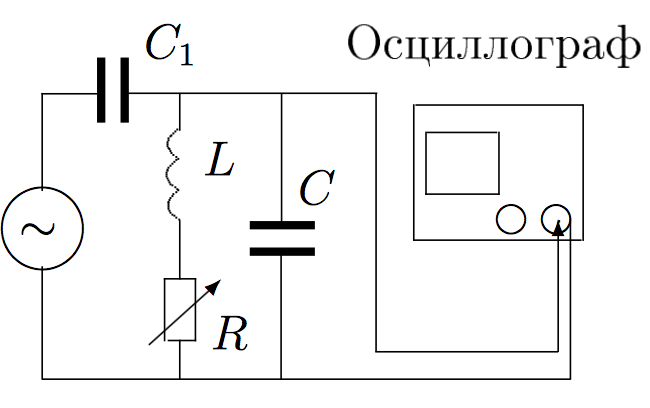
\includegraphics[width=5cm]{Scheme2}
\caption{Схема установки}
\end{wrapfigure} 

Мы можем снять зависимость амплитуды напряжения на резисторе $R$ от частоты на генераторе (при постоянной амплитуде выходного напряжения), однако для этого выходное сопротивление генератора должно быть много меньше импеданса контура. Для этого в цепи используется конденсатор $C_1$. И в таком случае импеданс внешней по отношению к контуру цепи был гораздо больше импеданса самого контура вблизи резонанса:

$$\dfrac{1}{\omega C_1} \gg |Z_\text{рез}| = \dfrac{L}{RC} $$

\subsection{Процессы установления и затухания колебаний}

\begin{wrapfigure}[12]{l}{7cm}
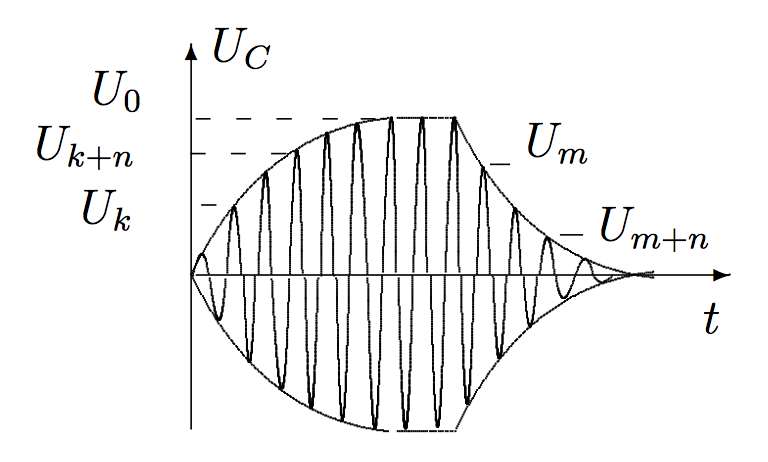
\includegraphics[width=7cm]{Scheme3}
\caption{Нарастание и затухание вынужденных колебаний}
\end{wrapfigure} 

Добротность контура можно определить и другими способами, например, по скорости затухания свободных колебаний. Подавая на контур цуги синусоид конечной длины, можно наблюдать процессы установления и затухания колебаний в контуре. И те, и другие могут быть использованы для определения добротности контура по скорости нарастания/затухания напряжения:

$$\Theta = \dfrac{1}{n} \ln \dfrac{U_0 - U_k}{U_0-U_{k+n}} $$


Измеряя амплитуды напряжения в какой-нибудь момент времени и через n периодов, можем посчитать добротность по формуле:
$$Q = \dfrac{\pi}{\gamma 	T} = \dfrac{\pi}{\Theta}$$
\section{Установка и параметры измерения}

\begin{figure}[H]
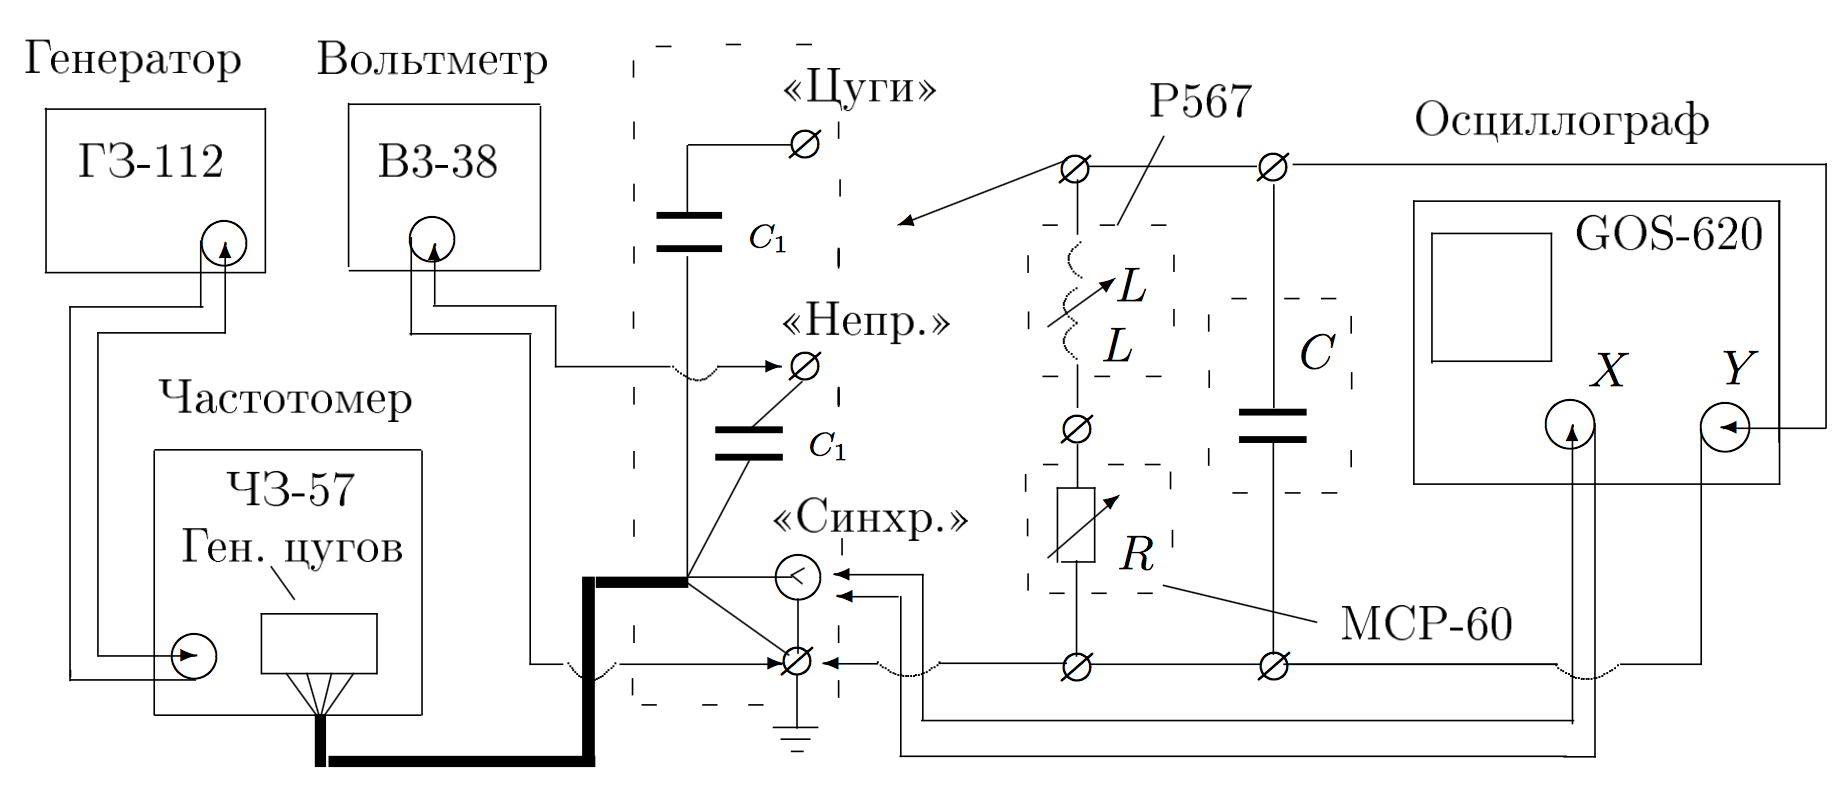
\includegraphics[width = 0.9 \tw]{Scheme}
\caption{Схема экспериментальной установки для исследования вынужденных колебаний}
\end{figure}

Идеальная схема, изображённая на рисунке 2, не соответствует действительности.  Элементы цепи не идеальны и имеют паразитные сопротивления. Измерим все величины с помощью RLC – моста:

$$R_L = 24.6 \; \Ohm,\; L = 99.97 \; \sm \H, \; C = 103.34 \; \sn \F, \; R = 105.7 \; \Ohm$$

Снимем зависимость напряжения на конденсаторе от входной частоты, и получим таким образом резонансную кривую. Рассчитаем добротность контура при разных значениях резистора по известной формуле:

$$Q = \dfrac{\nu_0}{\Delta \nu}$$

\begin{table}[H]
\centering
\resizebox{\textwidth}{!}{
\begin{tabular}{|c|c|c|c|c|c|c|c|c|c|c|c|c|c|c|c|c|c|c|c|c|c|c|}
\hline
U, \V  & 4.10  & 4.40  & 4.90  & 5.40  & 6.00  & 6.80  & 7.80  & 8.60  & 9.50  & 9.80  & 9.80  & 9.00  & 8.40  & 7.20  & 6.60  & 9.90  & 9.60  & 9.40  & 9.70  & 9.70  & 9.60  & 9.80  \\ \hline
$\nu$, \hz & 1575  & 1584  & 1588  & 1591  & 1595  & 1600  & 1605  & 1609  & 1615  & 1624  & 1636  & 1566  & 1562  & 1560  & 1556  & 1553  & 1550  & 1546  & 1541  & 1535  & 1527  & 1517  \\ \hline
$\nu/ \nu_0$  & 0.99  & 1.00  & 1.00  & 1.00  & 1.00  & 1.01  & 1.01  & 1.01  & 1.01  & 1.02  & 1.03  & 0.98  & 0.98  & 0.98  & 0.98  & 0.98  & 0.97  & 0.97  & 0.97  & 0.96  & 0.96  & 0.95  \\ \hline
U/U0  & 0.41  & 0.44  & 0.49  & 0.55  & 0.61  & 0.69  & 0.79  & 0.87  & 0.96  & 0.99  & 0.99  & 0.91  & 0.85  & 0.73  & 0.67  & 1.00  & 0.97  & 0.95  & 0.98  & 0.98  & 0.97  & 0.99  \\ \hline
$\Delta \nu/ \nu_0$ & 6.22  & 6.25  & 6.27  & 6.28  & 6.30  & 6.32  & 6.34  & 6.35  & 6.38  & 6.41  & 6.46  & 6.18  & 6.17  & 6.16  & 6.14  & 6.13  & 6.12  & 6.10  & 6.08  & 6.06  & 6.03  & 5.99  \\ \hline
$\Delta U/U0$ & 0.002 & 0.002 & 0.002 & 0.002 & 0.002 & 0.002 & 0.003 & 0.003 & 0.003 & 0.003 & 0.003 & 0.003 & 0.003 & 0.002 & 0.002 & 0.003 & 0.003 & 0.003 & 0.003 & 0.003 & 0.003 & 0.003 \\ \hline
\end{tabular}%
}
\caption{Полученные значения при R = 0}
\end{table}

\begin{figure}[H]
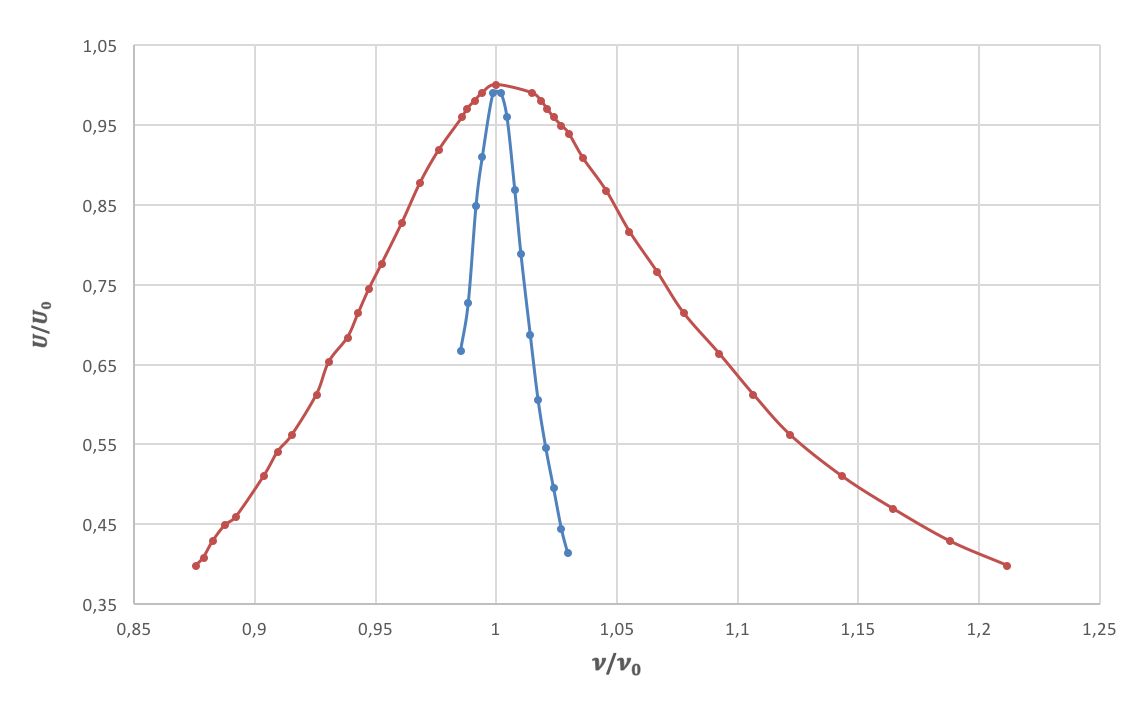
\includegraphics[width = 0.9 \tw]{Graph1}
\caption{Резонансные кривые для $R = 100 \; \Ohm$ и для $R = 0 \; \Ohm$}
\end{figure}

\subsubsection*{Экспериментальные значения добротностей:}
\begin{gather*}
Q_{R=0} = 38.4 \pm 1.2 \\
Q_{R=100} = 7.3 \pm 0.4
\end{gather*}

\begin{table}[H]
\centering
\begin{tabular}{|c|c|c|c|c|c|c|c|c|}
\hline
                    & \multicolumn{4}{c|}{Возрастание} & \multicolumn{4}{c|}{Затухание}                    \\ \hline
$R, \; \Ohm$        & \multicolumn{3}{c|}{0}   & 100   & \multicolumn{2}{c|}{0} & \multicolumn{2}{c|}{100} \\ \hline
$U_{n}, \; \sm \V$  & 44     & 68     & 56     & 16    & 680        & 380       & 152         & 164        \\ \hline
$U_{k+n},\; \sm \V$ & 160    & 160    & 160    & 60    & 100        & 100       & 24          & 24         \\ \hline
$U_0, \; \sm \V$    & \multicolumn{3}{c|}{177} & 61    & \multicolumn{4}{c|}{-}                            \\ \hline
n                   & 25     & 23     & 23     & 6     & 25         & 17        & 5           & 5          \\ \hline
Q                   & 38.2   & 38.8   & 36.8   & 5     & 41         & 40        & 8.5         & 8.2        \\ \hline
\end{tabular}
\caption{Измерение добротности по нарастанию и затуханию}
\end{table}

\subsubsection*{Экспериментальные значения добротности (нарастание напряжения):}
\begin{gather*}
Q_{R=0} = 38 \pm 4 \\
Q_{R=100} = 5 \pm 2
\end{gather*}

\subsubsection*{Экспериментальные значения добротности (убывание напряжения):}
\begin{gather*}
Q_{R=0} = 40.5 \pm 3 \\
Q_{R=100} = 8.3 \pm 2
\end{gather*}

\subsection*{Сравнение экспериментальных значений добротности, полученных разными методами}

\begin{table}[H]
\centering
\begin{tabular}{|c|c|c|c|c|}
\hline
            & Теория & Резонансная кривая & Нарастание & Убывание     \\ \hline
$Q_{R=0}$   & 38.8   & $38.4 \pm 1.2$     & $38 \pm 4$ & $40.5 \pm 3$ \\ \hline
$Q_{R=100}$ & 7.51   & $7.3 \pm 0.4$      & $5 \pm 2$  & $8.3 \pm 2$  \\ \hline
\end{tabular}
\caption{Сравнение экспериментальных значений добротности, полученных разными методами}
\end{table}

\section{Вывод}
Были изучены законы, описывающие переходные процессы в резонансном контуре, изучена резонансная кривая и определение добротности из разных физических соображений.

\end{document}
